% flashcards-title: A dot on a number line between 3 and 4
% flashcards-desc: A horizontal number line with arrowheads on both ends. Tall marks labeled 3 and 4 bound the middle of the line, shorter equally spaced marks cut the space between them into ten equal steps, and a round dot sits on one of the marks between 3 and 4.
\documentclass[tikz]{standalone}
\usetikzlibrary{arrows.meta,patterns}

\definecolor{qraNavy}{HTML}{17324D}
\definecolor{qraBlue}{HTML}{2B6CB0}
\definecolor{qraGold}{HTML}{B7791F}
\definecolor{qraPale}{HTML}{EAF2F8}
\definecolor{qraGray}{HTML}{5C6773}

\tikzset{
  qra axis/.style={draw=qraNavy, line width=1.2pt},
  qra tick/.style={draw=qraNavy, line width=1pt},
  qra guide/.style={draw=qraGray, densely dashed, line width=0.8pt},
  qra counter/.style={circle, draw=qraNavy, fill=qraPale, line width=0.9pt, minimum size=7mm, inner sep=0pt},
  qra label/.style={font=\sffamily\bfseries, text=qraNavy},
  qra small label/.style={font=\sffamily, text=qraNavy},
}

\begin{document}
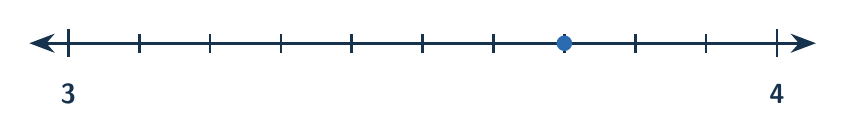
\begin{tikzpicture}[x=0.9cm]
  \draw[qra axis, {Stealth[length=3.2mm]}-{Stealth[length=3.2mm]}] (-0.55,0) -- (10.55,0);
  % Taller end marks at 3 and 4
  \draw[qra tick] (0,-0.18) -- (0,0.18);
  \draw[qra tick] (10,-0.18) -- (10,0.18);
  % Interior tenth marks
  \foreach \n in {1,...,9} \draw[qra tick] (\n,-0.12) -- (\n,0.12);
  \node[qra label, below=6pt] at (0,-0.18) {3};
  \node[qra label, below=6pt] at (10,-0.18) {4};
  % Dot on the seventh mark
  \fill[qraBlue] (7,0) circle (2.8pt);
\end{tikzpicture}
\end{document}
